\documentclass[12pt, a4paper]{article}
\usepackage{../notesheets}
%%%%%%%%%%%%%%%%%%%%%%%%%%%%%%%%%%%%%%%%%%%%%%%%%% 
\author{Math 1220}
\title{Notesheet. Section 8.3: Maxima and Minima of Function of
  Several Variables}
\date{}

\begin{document}
\maketitle
\nameline
%%%%%%%%%%%%%%%%%%%%%%%%%%%%%%%%%%%%%%%%%%%%%%%%%%
\vspace{-0.3in}
\begin{defi}
  Let \(f(x,y)\) be a function defined on a region \(R\) containing
  the point \((a,b)\). Then,
  \begin{itemize}
  \item \(f\) has a \de{relative maximum at \((a,b)\)} with
    \de{relative maximum value} \(f(a,b)\) if \\
    
  \item \(f\) has a \de{relative minimum at \((a,b)\)} with
    \de{relative minumum value} \(f(a,b)\) if\\
    
  \item \(f\) has an \de{absolute maximum at \((a,b)\)} with
    \de{absolute maximum value} \(f(a,b)\) if\\
    
  \item \(f\) has an \de{absolute minimum at \((a,b)\)} with
    \de{absolute minimum value} \(f(a,b)\)if
  \end{itemize}
\end{defi}
\begin{thrm}
  If \(f(x,y)\) is a differentiable function of two variables and has
  a relative maximum (relative minimum) at a point \((a,b)\) in the
  domain of \(f\), then 
\end{thrm}
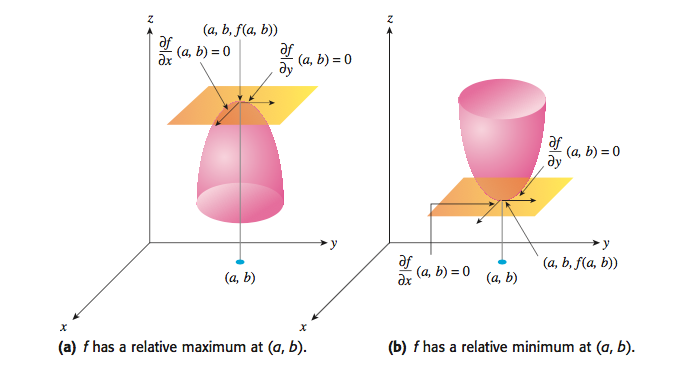
\includegraphics[scale=0.5]{images/local-min-max}
\begin{defi}
  A \de{critical point} is a point where 
\end{defi}
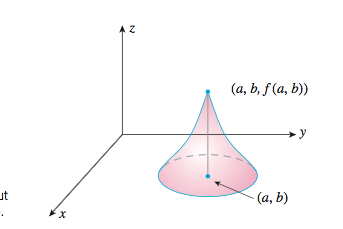
\includegraphics[scale=0.5]{images/critical-pt-deriv-dne} 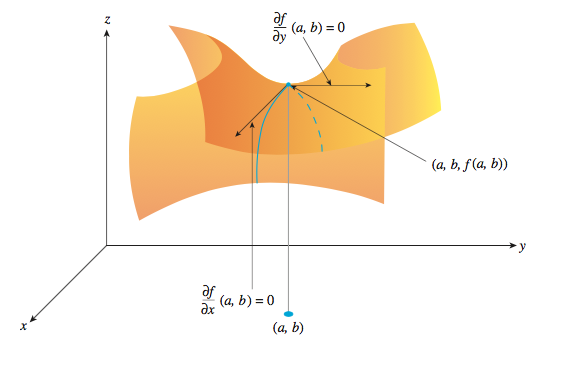
\includegraphics[scale=0.35]{images/saddle-point}
\begin{defi}
  A \de{saddle point} is a point where 
\end{defi}
\vspace{-0.1in}
\begin{ex}
  Consider the function \(f(x,y) = (1-x^2) \sin(y)\). Compute the
  following
  \begin{enumerate}
  \item \(f_x(0,0), f_y(0,0)\) and \(f_x(1,0),f_y(1,0)\).
    \vspace{0.75in}
  \item \(f_{xx}(0,0), f_{xy}(0,0), \) and \(f_{yy}(0,0)\)
    \vspace{0.75in}
  \item \(f_{xx}(1,0), f_{xy}(1,0),\) and \(f_{yy}(1,0)\)
  \end{enumerate}
\end{ex}
\vspace{-1.5in}
\begin{thrm}[The Second Derivative Test]
  Let \(f(x,y)\) be a twice differentiable function with continuous
  second derivatives. Let \[
    D(a,b) = f_{xx}(a,b)f_{yy}(a,b) - [f_{xy}(a,b)]^2
  \]
  If \(f_x = 0\) and \(f_y = 0\),
  \begin{enumerate}[label=(\alph*)]
  \item \(D(a,b) > 0\) and \(f_{xx}(a,b) < 0\), then
    \vspace{0.075in}
  \item \(D(a,b) > 0\) and \(f_{xx}(a,b) > 0\), then
    \vspace{0.075in}
  \item \(D(a,b) < 0\), then
    \vspace{0.075in}
  \item \(D(a,b) = 0\), then
  \end{enumerate}
\end{thrm}
\vspace{-0.5in}
%%%%%%%%%%%%%%%%%%%%%%%%%%%%%%%%%%%%%%%%%%%%%%%%%% 
\end{document}
